\documentclass[a4paper]{article}

\usepackage[spanish]{babel} 
\usepackage[utf8]{inputenc} 
\usepackage[T1]{fontenc}

\usepackage[a4paper,top=2.5cm,bottom=2.5cm,left=2.5cm,right=2.5cm]{geometry}

\usepackage{amsmath,amsthm, amssymb} 
\usepackage{graphicx} 
\usepackage{hyperref}
\usepackage{graphicx, graphics}
\usepackage{listings}

\newtheorem{theorem}{Teorema}
\newtheorem*{remark}{Observación}
\newtheorem{definition}{Definición}
\newtheorem{proposition}{Proposición}
\newtheorem{lemma}{Lema}

\lstset{%
    language=Python,                % Establecer lenguaje de programación
    basicstyle=\ttfamily\small,      % Estilo de la fuente
    mathescape=true                  % Permite usar matemáticas en el código
}

\title{Graph Counterfactual Explanation} 
\author{Kevin Manzano Rodr\'iguez \\ Roger Fuentes Rodr\'iguez} 
\date{}

\begin{document}

\maketitle

\section{Introducción}
En este trabajo, exploramos un modelo de aprendizaje automático (ML) que recibe grafos como entrada, denominado caja negra \(M\). Específicamente, nos enfocamos en el problema de búsqueda de contrafactuales, que consiste en encontrar una perturbación \(G'\) a partir de un grafo inicial \(G\) tal que las salidas del modelo para ambas entradas sean diferentes.

\section{Definición del Problema}

Nuestro objetivo es identificar contrafactuales "buenos", es decir, aquellos que son cercanos a \(G\). Formalmente, dado un modelo \(M\) y un grafo \(G\), buscamos devolver \(G'\) lo más cercano posible a \(G\) cumpliendo con la condición de que las salidas del modelo para \(G\) y \(G'\) sean distintas. Nos referimos a cercano con la m\'etrica de \textbf{edit distance}, b\'asicamente se tienen ambos grafos y se cuentan la cantidad de aristas que est\'an en diferentes estados.
 $$ED(G, G') = \sum_{e \in E(G) \wedge  e \notin E(G')}1  + \sum_{e \in E(G') \wedge  e \notin E(G)} 1$$

Definimos como perturbación de un grafo $G$ a $G'$ si $G'$ puede ser obtenido a partir de $G$ mediante perturbaciones en las aristas, en donde perturbar una arista significa cambiar el estado de la misma, si $e \in G$ y la perturbamos luego $e \notin G$ y viceversa. Notemos que desde cualquier grafo podemos ir a cualquier otro, entonces podemos pensar en el grafo de todos los posibles grafos de $n$ nodos como un grafo completo de $2 ^ {\binom{n}{2}}$ nodos, con pesos en las aristas que representan la cantidad de aristas que se necesitan perturbar para llegar de uno a otro de forma directa (no tiene sentido perturbar dos veces una arista).

Luego tenemos un modelo que desconocemos que predice, al cual llamaremos or\'aculo y dado una entrada $G$ queremos encontrar $G'$ tal que cumple $M(G) \neq  M(G')$ y es m\'inimo o sea si existe otro $G''$ tal que $M(G) \neq  M(G'')$ entonces $ED(G, G') \leq ED(G, G'')$. Adem\'as se posee el dataset donde se encuentran todos los grafos de importancia

El proceso de b\'usqueda de contrafactuales se dividir\'a en dos partes \textbf{generate} y \textbf{minimizer}, la primera se centra en buscar un contrafactual, pero no asegura que sea m\'inimo, y la segunda se dedica a mejorar el contrafactual encontrado inicialmente.

Este problema usualmente es atacado con modelos de ML pero en nuestro caso se propone un algoritmo de aproximaci\'on (metaheur\'istica), se queda de estudio si es un \textbf{k-factor} .

\section{Metodolog\'ia}

Uno de los requisitos que se quieren mejorar es la cantidad de llamadas al or\'aculo debido a lo costosas que son, por lo que en ambas secciones se pretende minimizar las mismas. En nuestra primera secci\'on de b\'usqueda de minimizer se brinda una soluci\'on lineal en el tamaño del dataset con respecto a la cantidad de llamados al or\'aculo, asegurando un buen comienzo para el \textbf{minimizer} jugando con la geometr\'ia del espacio. Luego en nuestra segunda secci\'on se brinda un algoritmo de aproximaci\'on que tiene una componente probabil\'istica, que luego se mejorar\'a con m\'etodos de \textbf{taggeo} en aristas. Se brindan varios m\'etodos para etiquetar las aristas, se comentan curiosidades de problemas abiertos, teoremas importantes y soluciones cl\'asicas a problemas hermosos. Para la verificaci\'on de la eficiencia de las soluciones se cuenta con varios datasets.

\section{Generate}


Supongamos que tenemos todas las categorías existentes en nuestro dataset $C_1, C_2, ..., C_m$ y queremos generar un contrafactual para el grafo $G$ con el modelo $M$, si  $C_i$ es a la que pertenece $G$, un contrafactual v\'alido para $G$ con $M$ ser\'ia cualquier grafo que pertenece a $C_j$ con $j \ne i$. Tambi\'en ser\'ia bueno tener grafos cercanos de forma general a todos los grafos de la entrada, por lo que vamos a construir una idea de cercanía.

Dado una categor\'ia del $C$, formemos el subconjunto de los grafos del dataset que pertenecen a $C$ (realizando una llamada al or\'aculo podemos saber a que categor\'ia pertenece). Nos concierne encontrar un grafo especial intuitivamente cercano a todos los grafos de categor\'ias diferentes a $C$ (\textbf{memoide}), si se logra modelar los grafos como puntos en un espacio, entonces el problema se reducir\'ia a encontrar el punto que minimiza la distancia a todos los puntos de las categor\'ias diferentes.

Para modelar nuestro espacio vectorizamos los grafos de la siguiente forma, sea $G$ entonces tendremos $v$ un vector de $\binom{E(G)}{2}$ componentes donde los $x_i$ son binarios, $1$ si la arista $e$ en la posici\'on $i$ est\'a en $G$, $0$ en caso contrario, en donde el orden de las aristas esta dado por el orden de los par ordenado $(xy)$ que representan la arista $xy$ (aqui tomemos $x<y$ para desambiguar). Luego la distancia entre dos puntos equivale a $ED(G, G')$.

Entonces simplemente dado una categor\'ia $C$ el memoide de dicha categor\'ia ser\'a $G$ si y solo si $G \in C$ y si existe $G' \in C$ entonces $\sum_{G'' \notin C} ED(G, G'') \leq \sum_{G'' \notin C} ED(G', G'')$.

Luego podemos tener un grafo 'cercano' a cualquier grafo en cada una de las categor\'ias, por lo que obtener un contrafactual consistir\'a en iterar por todas las categor\'ias diferentes a la que pertenece el grafo en cuesti\'on y devolver el m\'as cercano a \'el.

Entonces tenemos una soluci\'on en $O(n^2)$ donde $n$ es el tamaño del dataset porque dado un grafo se itera por todos los dem\'as grafos que cumplen que est\'an en categor\'ias diferentes y se acumula la suma, y solo necesitamos llamar al or\'aculo $n$ veces, luego al entrar un grafo se hace una llamada m\'as al or\'aculo para saber cual es su categor\'ia y se busca en las categorias diferentes cual está m\'as cercano. Por lo que sabemos que hicimos la cantidad m\'inima de llamados al or\'aculo para dar un contrafactual sensato inicial, una idea podr\'ia haber sido iterar por el dataset en cada entrada e ir preguntando cual es el primero en una categor\'ia diferente, pero esto no es eficiente pues tendriamos varios llamados para un mismo grafo, y tambi\'en disminuimos la cantidad de iteraciones por entrada, solo a la cantidad de categor\'ias diferentes, aunque perdimos en eficiencia porque se podr\'ia devolver la primera diferente pero queremos mejorar en optimalidad del contrafactual en si manteniendo un balance porque se podr\'ia buscar directamente el m\'as cercano a la entrada.

\section{Minimizer}

\subsection{Local Search}

Sea $G = (V, E)$ un grafo genérico y un modelo de caja negra (u \emph{oráculo}) $M$ que clasifica o decide sobre $G$. 
Decimos que un \emph{contrafactual} para $G$ es un grafo $G'$ resultante de perturbar (insertar o eliminar) aristas en $G$ tales que la salida de $M$ con entrada $G'$ cambia con respecto a la salida de $M$ con entrada $G$.  
El problema \emph{GCE} (\emph{Graph Counterfactual Explanation}) pregunta: 

\begin{quote}
    \emph{¿Cuál es el número mínimo de aristas que deben perturbarse en $G$ para que el modelo $M$ cambie su decisión?}
\end{quote}

En términos de decisión, se formula como:

\begin{definition}[Problema de Decisión GCE]
Dado un grafo $G=(V,E)$, un entero $k$ y un oráculo $M$ que toma grafos como entrada,  
¿existe un conjunto de perturbaciones $S \subseteq E^+$
(\,$|S| \leq k$\,) 
tal que, al perturbar todas las aristas en $S$ y obtener $G'$, 
el oráculo $M$ cambie su salida con respecto a la que proporcionó al evaluar $G$?
\end{definition}

Aquí, $E^+$ es el conjunto de todas las aristas posibles (existentes o no) que podrían alterarse.

\subsection{Reducción desde FES}

Para probar que GCE es NP-Completo, se realiza una reducción polinomial desde el problema \emph{FES} (Conjunto de Aristas de Retroalimentación, por sus siglas en inglés). 

\begin{definition}[FES - Feedback Edge Set]
Sea $G=(V,E)$ un grafo no dirigido. 
Un \emph{FES} es un subconjunto $F \subseteq E$ tal que, al eliminar las aristas en $F$, el grafo se vuelve acíclico (un bosque).  
El problema de decisión asociado pregunta: \emph{dado un entero $k$, existe un conjunto $F$ con $|F|\leq k$ que elimine todos los ciclos en $G$?}
\end{definition}

Se sabe que FES es NP-completo (fue uno de los 21 problemas que Karp demostró NP-completos).

\subsubsection*{Teorema principal}

\begin{theorem}\label{thm:NP}
El problema GCE es NP-completo, pues FES se reduce a GCE.  
\end{theorem}

\begin{proof}[Demostración]
Sea $G$ un grafo no dirigido para el problema FES.  
Definimos un oráculo $M'$ que, dada una entrada $H$, responde:
\[
 M'(H) = 
 \begin{cases}
   \text{true}, & \text{si }H\text{ es acíclico;}\\
   \text{false}, & \text{en caso contrario.}
 \end{cases}
\]
Claramente, decidir si $H$ es acíclico o no está en NP.  
Mostraremos:

\[
\text{FES}(G,k) = \text{true} 
\quad \Longleftrightarrow \quad
\text{GCE}(G, k, M') = \text{true}.
\]

\paragraph{($\Rightarrow$) Si FES$(G,k) =$ true.}
Existe un conjunto $S \subseteq E$ con $|S|\leq k$ tal que eliminar $S$ de $G$ produce un grafo acíclico $G'$.  
Al presentar $G$ a $M'$, su salida es \texttt{false} (pues $G$ tenía ciclos).  
Al perturbar (eliminar) exactamente las aristas en $S$, obtenemos $G'$ sin ciclos.  
Entonces $M'(G') = \texttt{true}$.  
Por definición, esto es un contrafactual para $G$ con a lo sumo $k$ perturbaciones.  
Así, GCE$(G,k,M') = \texttt{true}$.

\paragraph{($\Leftarrow$) Si GCE$(G, k, M') =$ true.}
Existe un conjunto de perturbaciones $S$ con $|S| \leq k$ que convierte $G$ de cíclico a acíclico (pues la salida de $M'$ cambia de \texttt{false} a \texttt{true}).  

\begin{lemma}\label{lemma:eliminar_aristas}
Si en las perturbaciones de $S$ hay inserciones de aristas, podemos descartarlas sin afectar el cambio de \texttt{false} a \texttt{true}. 
\end{lemma}
\begin{proof}[Idea de la demostración]
Agregar aristas no ayuda a eliminar ciclos; si el grafo $G'$ final es acíclico con inserciones y eliminaciones, basta quitar las inserciones para quedarse sólo con las eliminaciones, manteniéndose acíclico.  
\end{proof}

En consecuencia, podemos obtener un subconjunto $S'\subseteq S$ (solo eliminaciones) tal que $|S'|\le k$ y $G\setminus S'$ sea acíclico.  
Esto corresponde exactamente a la solución FES$(G,k)=\texttt{true}$.  

\noindent
Por tanto, existe reducción polinomial de FES a GCE.  
Al estar FES en NP-completo, concluimos que GCE es NP-completo.  

\end{proof}

\section{Metaheurística de Búsqueda Local}

Para aproximar la solución de GCE (dado que es NP-completo), se propone una metaheurística basada en \emph{búsqueda local}.  
En particular, se emplea \textbf{Búsqueda de Vecindad Variable (VNS)}, cuyas ideas clave son:

\begin{itemize}
    \item \textbf{Definición de solución:} 
    Una solución es un subconjunto de aristas perturbadas (insertadas/eliminadas).
    \item \textbf{Vecindarios:} 
    Se contemplan tres criterios de vecindad principales sobre la solución actual $S$:
    \begin{enumerate}
        \item Reemplazar aristas en $S$ por otras que no están en $S$. 
        \item Eliminar aristas de $S$. 
        \item Agregar nuevas aristas que no estén en $S$. 
    \end{enumerate}
    \item \textbf{Estrategia de VNS:} 
    \begin{enumerate}
        \item Iniciar con una solución factible (un contrafactual cualquiera, posiblemente grande).  
        \item Cambiar sistemáticamente de vecindad cuando no se consiguen mejoras (o cuando se encuentran mínimos locales).  
        \item Si se encuentra una mejor solución en una vecindad, se actualiza la solución actual y se regresa al vecindario más pequeño.  
        \item Repetir hasta criterio de parada (tiempo, número de iteraciones sin mejora, etc.). 
    \end{enumerate}
    \item \textbf{Aceptación de mejoras:} 
    Por lo general se adopta la primera mejora (\emph{first improvement}) o la mejor mejora (\emph{best improvement}) en cada vecindario.
\end{itemize}

\subsection{Label Edge}

Para mejorar la componente aleatoria al seleccionar aristas que perturbar vamos a presentar varios etiquetados de aristas como algoritmo goloso para en cada entrada en dependencia de las caracter\'isticas del modelo y del grafo, seleccionar uno de los etiquetados. El algoritmo inicialmente utilizaba el etiquetado trivial, al ordenarlas en dependencia de los pares que representan la arista tomando al menor como comienzo.

\subsubsection{Etiquetado Elegante}

A modo cultural presentamos este etiquetado de vertices. Este etiquetado conocido como \textbf{graceful labeling} se basa en una inyecci\'on de los vertices en el conjunto $\{0, 1, ..., E(G)\}$ tal que $e=uv$ recibe la etiqueta $|u - v|$, notemos que los valores de las aristas est\'an entre 1 y $E(G)$, ahora si las etiquetas de las aristas son \'unicas entonces el grafo recibe el nombre de \textbf{graceful}.

Un problema abierto en teor\'ia de grafos es la conjetura de Ringel-Kotzig o  \textbf{graceful tree}, la cual dice que todos los \'arboles son graceful.

Alexander Rosa demostr\'o que las grafos eulerianos con un n\'umero de aristas $m \equiv 1, 2 (4)$ no pueden ser graceful, adem\'as demostro que $C_n$ es graceful si y solo s\'i $n \equiv 0,3 (4)$.

Similar a esta forma de etiquetar se tiene tambi\'en su an\'alogo \textbf{edge graceful labeling} que consiste en dado un etiquetado de las aristas , los v\'ertices son etiquetados de la siguiente forma:
$$ V(u) = \sum_{u \in e} E(e) \mod V(G)$$

El problema consiste en buscar una forma de asignar etiquetas a las aristas que cumple que las etiquetas de las aristas son un subconjunto de $\{1,2, ..., E(G)\}$ y las etiquetas de los v\'ertices son un subconjunto de $\{0, 1, ..., V(G)-1\}$.

Aqu\'i se tiene un buen resultado una condicion necesaria para que un grafo sea edge-graceful debe cumplir que si $q = E(G)$ y $p = V(G)$ entonces:
$$q(q+1) \equiv \frac{p(p-1)}{2} \mod p$$

Esto sale del hecho que la suma de las etiquetas de los v\'ertices es dos veces la suma de las etiquetas de las aristas.

Tambi\'en se tiene \textbf{Harmonious labeling} de un grafo es una inyecci\'on de los v\'ertices al grupo de enteros mod  $k$, donde $k$ es el n\'umero de aristas, que induce una biyecci\'on entre las aristas de $G$ y los n\'umeros mod $k$, donde a la arista $e=uv$ se le asigna $v+u \mod k$. Est\'a conjeturado que los \'arboles son todos harmoniosos si una de las etiquetas de los v\'ertices tiene permitido ser reusada.

\subsubsection{Coloraci\'on de Aristas}
 Un problema conocido es el coloreo de grafos, ya sea en v\'ertices o en aristas, en nuestro caso nos concierne solo las aristas, queremos etiquetar las aristas de forma que si dos aristas comparten alg\'un extremo entonces tengan colores diferentes. Se quiere minimizar la cantidad de colores diferentes usados.


 Comencemos creando unas ideas iniciales. Sea $D = max_{v \in V(g)}deg(v)$ o sea el mayor de los grados del grafo, dado que las aristas de un mismo v\'ertice tienen que tener todas colores diferentes entonces, no se puede colorear con menos de $D$ colores. Por lo que si de alguna manera podemos colorear el grafo con $D$ colores esta ser\'a m\'inima. Esto obviamente no es cierto consideremos $C_3$, tendr\'iamos $D = 2$ y no funcionar\'ia, necesitamos $D+1$ colores. De hecho tenemos el teorema de Vizing, que expresa que un grafo simple se puede colorear las aristas con a lo sumo $D + 1$ colores, por lo que habran dos clases de grafos, los que necesitan $D$ y los que necesitan $D+1$, existe una versi\'on m\'as general para multigrafos que es muy similar lo que requiere de la multiplicidad, se necesitan a los sumo $D + m$ donde $m$ es la multiplicidad del multigrafo.

 Aun cuando casi todos los grafos pertenecen a la clase 1 (Erdos y Wilson $lim_{n \rightarrow  \infty} \frac{|G_n^1|}{|G_n|} = 1$) con los bipartitos incluidos (Koning) resulta que es Np completo el problema de decisi\'on si $G$ admite un $k-edge$ coloreo.

 Demostremos el caso de grafos simples (Vizing)

 Sea $f$ un coloreo de aristas propio de $D + 1$ colores de un subgrafo $G'$ de $G$. Si $G' \neq G $ entonces alguna arista $uv$ no est\'a coloreada por $f$. Despu\'es posiblemente recoloreando algunas aristas podemos extender nuestro coloreo para incluir $uv$, llamemos a esto un aumento. Despu\'es de $e(G)$ aumentos, obtenemos un coloreo propio de $D + 1$ colores. 
 
 Dado que el n\'umero de colores excede $D$, se cumple que para todo v\'ertice se tiene al menos un color que no aparece en sus aristas incidentes. Sea $a_0$ un color faltante en $u$. Generemos una lista de vecinos de $u$ y una lista correspondiente de colores. Empezemos con $v_0 = v$.
 
 Sea $a_1$ el color faltante en $v_0$. Podemos asumir que $a_1$ aparece en $u$ en alguna arista $uv_1$, de otra forma podemos utilizar $a_1$ en $uv_0$.
 
 Sea $a_2$ el color faltante en $v_1$. Podemos asumir que $a_2$ aparece en $u$ en alguna arista $uv_2$, de otra forma podemos reemplazar el color $a_1$ con $a_2$ en $uv_1$ y luego usar $a_1$ en $uv_0$ para aumentar el coloreo. 
 
 Teniendo seleccionado $uv_{i-1}$ con el color $a_{i-1}$, sea $a_i$ el color faltante en $v_{i-1}$. Si $a_i$ est\'a faltante en $u$ entonces usamos $a_i$ en $uv_{i-1}$ y corremos el color $a_j$ desde $uv_j$ hasta $uv_{j-1}$ para $1 \leq j \leq i-1$ para completar el aumento. Llamemos un corrimiento para abajo desde $i$ a esto. Si $a_i$ aparece en $u$ (en alguna arista $uv_i$), entonces el proceso continua.

 Ver figura 1
 
\begin{figure}
    \begin{center}
        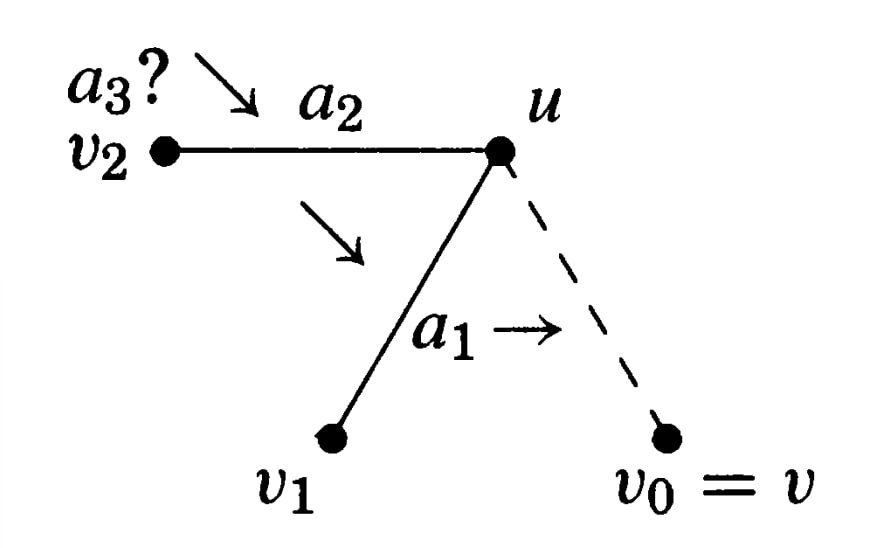
\includegraphics[width=8cm]{image1.png}
        \caption{Vizing theorem procedure} 
    \end{center}
\end{figure}

Dado que solo tenemos $D + 1$ colores para escoger, la lista de colores seleccionados ser repite eventualmente (o completamos el aumento por el corrimiento para abajo).

Sea $l$ el menor \'indice tal que el color faltante en $v_l$ esta en la lista $a_1, ..., a_l$, sea este color $a_k$. En cambio de extender la lista, usemos esta repetici\'on para aumentar en uno o muchos.

El color $a_k$ faltante en $v_l$ est\'a tambi\'en faltante en $v_{k-1}$ y aparece en la arista $uv_k$. Si $a_0$ no aparece en $v_l$, entonces podemos hacer un corrimiento para abajo desde $v_l$ y usar el color $a_0$ en $uv_l$ para crear un aumento. Dado que asumimos que $a_0$ aparece en $v_l$.

Sea $P$ el camino maximal alternante de aristas coloreadas con $a_0$ y con $a_k$ que empiezan en $v_l$ empezando con $a_0$. Solo hay un \'unico camino con esas caracter\'isticas porque cada v\'ertice tiene a lo sumo una arista incidente de cada color (ignoremos las aristas que no est\'an coloreadas). Para completar el aumento vamos a intercambiar los colores $a_0$ y $a_k$ en $P$ y corremos hacia abajo de forma apropiada a los vecinos de $u$, en dependencia de por donde va $P$.

Si $P$ alcanza $v_k$, entonces llega a $v_k$ a lo largo de aristas con color $a_0$, siguiendo $v_ku$ con color $a_k$, y para en $u$, lo que deja el color $a_0$. En este caso corremos para abajo desde $v_k$ y cambiamos los colores en $P$ (Ver figura 2 Izquierda)

Si $P$ alcanza $v_{k-1}$, entonces alcanza $v_{k-1}$ en el color $a_0$ y para all\'i, porque $a_k$ no aparece en $v_{k-1}$. En este caso hacemos un corrimiento para abajo desde $v_{k-1}$, le damos el color $a_0$ a $uv_{k-1}$ y cambiamos los colores en $P$ (Ver figura 2 Medio).

Si $P$ no alcanza $v_k$ o $v_{k-1}$, entonces el termina en alg\'un vertice fuera de $\{u, v_l, v_k, v_{k-1}\}$. En este caso hacemos un corrimiento para abajo desde $v_l$, le damos el color $a_0$ a $uv_l$ y cambiamos los colores en $P$ (ver figura 2 Derecha).
\begin{figure}
    \begin{center}
        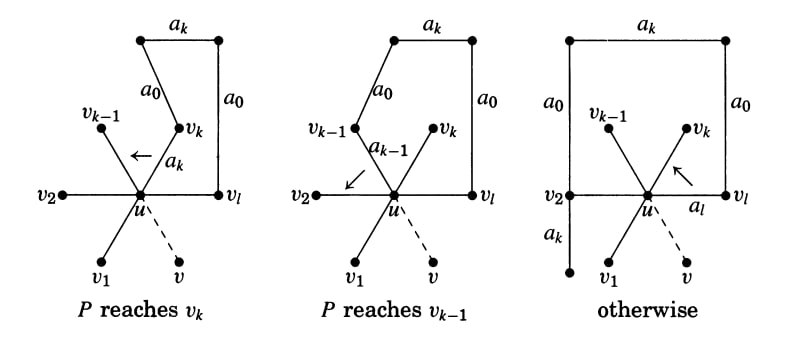
\includegraphics[width=8cm]{image2.png}
        \caption{Cada caso de $P$} 
    \end{center}
\end{figure}
En cada caso, los cambios descritos mantienen el coloreo propio de $D+1$ colores de $G + uv$, as\'i que completamos el aumento.

Consideramos el siguiente problema de decisión:

\begin{definition}[Problema de Coloración de Aristas]
Dado un grafo $G=(V,E)$ y un entero $k$, determinar si existe una función
\[
f : E \to \{1,2,\dots,k\}
\]
tal que para todo vértice $v\in V$, las aristas incidentes en $v$ tienen colores distintos.
\end{definition}

En particular, es conocido que para grafos generales (por ejemplo, para grafos cúbicos) el problema de decidir si un grafo admite una coloración de aristas con $k$ colores es NP-completo. En el caso de grafos cúbicos, por el teorema de Vizing se tiene que el número cromático de aristas es $3$ o $4$, por lo que decidir si existe una coloración con $3$ colores (es decir, si el grafo es de \emph{Clase 1}) es NP-completo (ver Holyer, 1981).

\begin{theorem}
El problema de determinar si un grafo $G$ admite una coloración de aristas con $k$ colores es NP-completo.
\end{theorem}

\begin{proof}
La demostración se divide en dos partes: (1) demostrar que el problema está en NP y (2) probar ques es NP-duro.

\textbf{(1) El problema está en NP:}\\
Sea la instancia $\langle G,k \rangle$. Un certificado natural es una asignación 
\[
f : E \to \{1,2,\dots,k\}.
\]
Dado dicho certificado, se puede verificar en tiempo polinómico que:
\begin{itemize}
    \item Para cada arista $e\in E$, se tiene que $f(e)\in \{1,2,\dots,k\}$.
    \item Para cada vértice $v\in V$, si se denota
    \[
    C(v)=\{ f(e) \mid e \text{ incide en } v \},
    \]
    se cumple que el tamaño de $C(v)$ es igual al número de aristas incidentes en $v$ (es decir, no hay dos aristas incidentes en $v$ con el mismo color).
\end{itemize}
Ambos pasos requieren recorrer los conjuntos de aristas y vértices, por lo que la verificación es polinomial. Por ello, el problema está en NP.

\vspace{0.3cm}
\textbf{(2) NP-dureza:}\\
La NP-dureza se demuestra mediante una reducción desde el problema de 3-coloración de aristas en grafos cúbicos, el cual es NP-completo (véase Holyer, 1981).

Sea $G$ un grafo cúbico, es decir, un grafo en el cual cada vértice tiene grado 3. Por el teorema de Vizing, la cantidad de colores necesaria para colorear las aristas de $G$ es 3 o 4. Entonces, el problema de decidir si $G$ es 3-colorable (es decir, si admite una coloración de aristas con 3 colores) es equivalente a determinar si $G$ es de \emph{Clase 1}. La reducción es directa, ya que la instancia del problema de 3-coloración de aristas es el mismo grafo $G$ junto con $k=3$. Dado que este problema se ha probado NP-completo, se concluye que el problema de coloración de aristas (en su versión de decisión) es NP-difícil.

\end{proof}

Para demostrar que es NP-duro se reduce 3-SAT a la 3-coloración de aristas en grafos cúbicos. La idea general es construir, a partir de una fórmula booleana $\phi$ en forma normal conjuntiva, un grafo cúbico $G_\phi$ tal que:
\[
\phi \text{ es satisfacible} \quad\Longleftrightarrow\quad G_\phi \text{ es 3-colorable en aristas.}
\]

La reducción se realiza en tres pasos principales:

\begin{enumerate}
    \item \textbf{Construcción de Gadgets de Variable:}  
    Para cada variable $x_i$ de la fórmula $\phi$, se diseña un gadget que admite exactamente dos coloraciones válidas. Estas dos coloraciones se interpretan como las asignaciones de \emph{verdadero} o \emph{falso} para la variable $x_i$. Además, el gadget se conecta con los gadgets de cláusula de forma que la elección de la coloración imponga restricciones sobre los colores en las conexiones.

    \item \textbf{Construcción de Gadgets de Cláusula:}  
    Para cada cláusula $(\ell_1 \lor \ell_2 \lor \ell_3)$, se construye un gadget que se conecta a los gadgets correspondientes a los literales $\ell_1$, $\ell_2$ y $\ell_3$. El gadget de cláusula se diseña de tal manera que una coloración válida (es decir, una asignación de colores a sus aristas) es posible si y solo si al menos uno de los literales es interpretado como \emph{verdadero}.

    \item \textbf{Conectores y Ajustes para Garantizar la Cubicidad:}  
    Se incorporan gadgets auxiliares o estructuras de conexión que aseguren que el grafo resultante es cúbico (cada vértice tiene grado 3) y que la transformación se efectúa en tiempo polinómico.
\end{enumerate}

\paragraph{Gadget de Variable:}  
El gadget asociado a cada variable $x_i$ está diseñado para que tenga exactamente dos posibles coloraciones (por ejemplo, asignando a algunas aristas el color 1 o el color 2 de forma forzada) y que estas dos coloraciones correspondan a la elección de $x_i=\text{verdadero}$ o $x_i=\text{falso}$. La conexión de este gadget con los gadgets de cláusula se hace mediante "puentes" que transfieren la información de la elección de la variable a la cláusula.

\paragraph{Gadget de Cláusula:}  
El gadget de cláusula está construido para que, si los tres literales de la cláusula resultan falsos (lo que se reflejaría en la imposibilidad de asignar los colores correctamente en el gadget), entonces no se podrá extender a una coloración válida del grafo completo. Por lo tanto, la existencia de una 3-coloración en aristas para el grafo construido implica que cada cláusula tiene al menos un literal verdadero.

La construcción del grafo $G_\phi$ satisface lo siguiente:
\begin{itemize}
    \item \textbf{Si $\phi$ es satisfacible:}  
    Dada una asignación que satisface $\phi$, se puede escoger la coloración correspondiente en cada gadget de variable. Luego, usando las restricciones impuestas por los gadgets de cláusula y los conectores, se extiende esta asignación a una coloración válida de aristas con 3 colores en todo el grafo $G_\phi$.
    
    \item \textbf{Si $G_\phi$ es 3-colorable en aristas:}  
    A partir de una coloración válida se puede inferir una asignación de valores a las variables. En efecto, la estructura de los gadgets garantiza que, para cada cláusula, al menos uno de los literales debe ser asignado de forma que la cláusula se satisfaga.
\end{itemize}

Como la transformación de una fórmula $\phi$ a un grafo cúbico $G_\phi$ se realiza en tiempo polinómico, la existencia de un algoritmo polinómico para 3-coloración de aristas implicaría un algoritmo polinómico para 3-SAT, lo cual es un absurdo bajo la hipótesis \(P \neq NP\).

Volviendo al problema inicial como tenemos grafos generales tendremos que dar una soluci\'on aproximada que encuentra un coloreo de $D+1$ colores. En caso de que se pudiera asegurar que todos los grafos son bipartitos, existe una forma de resolver el problema coloreando con $D$ colores utilizando flujo m\'aximo con lowerbound.

Ahora veamos un algoritmo que trabaja en $O(nm)$ para encontrar un coloreo de a lo sumo $D+1$ colores aprovechandose del teorema de Vizing, este algoritmo fue descrito por Misra y Gries. Un algoritmo mas r\'apido que
corria en $O(m\sqrt{nlogn})$ fue prometido en 1985 por Gabow pero nunca fue publicado.

Definamos un par de conceptos primero.

\begin{itemize}
    \item Color libre: Un color $c$ es libre en $u$ si no hay ninguna arista incidente en $u$ con el color $c$.
    \item Ventilador: Un ventilador en un v\'ertice $X$ es una secuencia de v\'ertices $F[1:k]$ que satisface las siguientes condiciones:
        \begin{itemize}
            \item $F[1:k]$ es una secuencia no vac\'ia de vecinos distintos de $X$
            \item La arista $XF[1]$ no est\'a coloreada
            \item El color de $XF[i+1]$ est\'a libre en $F[i]$ para $1 \leq i < k$
        \end{itemize}
        Dado un ventilador $F$, cualquier arista $XF[i]$ para $1 \leq i \leq k$ es una arista de ventilador.
    \item Rotar un ventilador: Dado un ventilador $F[1:k]$ de un v\'ertice $X$, la operaci\'on de rotar el ventilador hace lo siguiente: $for i=1,...,k-1$ asigna el color de $XF[i+1]$ a la arista $XF[i]$ y descolorea $XF[k]$. Esta operaci\'on deja un coloreo v\'alido debido a la definici\'on de ventilador, el color de $XF[i+1]$ est\'a libre para $F[i]$
    \item cd-path: La operaci\'on invertir el $cd_x-path$ cambia cada arista del camino coloreado $c$ a $d$ y cada arista coloreada $d$ a $c$. Invertir un camino puede ser \'util para liberar un color en $X$ si $X$ es uno de los extremos del camino: Si el color $c$ pero no $d$ es incidente en $X$, ahora el color $d$ pero no $c$ es incidente en $X$, liberando a $c$ de $X$. Esta operaci\'on deja un coloreo v\'alido. Para v\'ertices en el camino que no son extremos, ning\'un color es agregado. Para extremos, la operaci\'on cambia de color uno de sus aristas entre $c$ y $d$. Esto es v\'alido: supongamos que el extremo estaba conectado por una $c$ arista, entonces $d$ fue liberado en ese extremo, porque en otro caso, este v\'ertice no pod\'ia ser un extremo. Puesto que $d$ era libre, esta arista cambia a $d$.
\end{itemize}

\begin{lstlisting}
    Misra & Gries 
    input: Grafo G.
    output: Un coloreo propio c de las aristas del grafo G.

    Sea U := E(G)

    while U $\neq$ $\empty$ do
        Sea (X,v) una arista en U.  
        Sea F[1:k] un ventilador maximal de X con F[1]=v.
        Sea c un color libre en X y d un color libre en F[k].  
        Invertimos el cd_X-path.  
        Sea w $\in$ {1..k} tal que F`=F[1:w]
        es un ventilador y d esta libre en F[w].  
        Rotate F`.
        Establece el color de (X,w) a d.
        U := U - {(X,v)}
    end while
\end{lstlisting}

La correctitud del algoritmo se demuestra en tres partes, primero se demuestra que la inversi\'on de un camino $cd_x-path$ garantiza un $w \in \{1,...,k\}$ tal que $F' = F[1:w]$ es un ventilador y $d$ est\'a libre en $F[w]$. Entonces se demuestra que el coloreo de aristas es v\'alido y luego que requiere $D+1$ colores.

Caso 1: El ventilador no tiene aristas coloreadas $d$. Puesto que $F$ es un ventilador maximal de $X$ y $d$ est\'a libre en $F[k]$, entonces $d$ est\'a libre en $X$. De otra forma supongamos que una arista $Xu$ tiene el color $d$, entonces $u$ puede ser agregado a $F$ para hacer un ventilador m\'as grande contradiciendo el hecho de que $F$ era maximal. Por lo que $d$ est\'a libre en $X$, y dado que $c$ tambi\'en esta libre en $X$, entonces no existe $cd_x-path$ y la inversi\'on no tiene efecto en el grafo, establece $w = k$.

Caso 2: el ventilador tiene una arista con color \( d \). Sea \( (X, F[i+1]) \) esta arista. Observa que \( i+1 \neq 1 \) ya que \( (X, F[1]) \) no está coloreado. Por definición de un ventilador, \( d \) es libre en \( F[i] \). Además, \( i \neq k \) ya que el ventilador tiene longitud \( k \), pero existe un \( F[i+1] \). Ahora podemos demostrar que después de la inversión,
\[
(1): \quad \text{for} \, j \in \{1, \dots, k-1\} \setminus \{i\}, \, \text{el color de} \, (X, F[j+1]) \, \text{es libre en} \, F[j].
\]


Notemos que antes de la inversión, \( c \) es libre en \( X \) y \( (X, F[i+1]) \) tiene color \( d \), por lo que las otras aristas en el ventilador, es decir, todos \( (X, F[j+1]) \) arriba, no pueden tener color \( c \) ni \( d \). Dado que la inversión solo afecta a las aristas que están coloreados con \( c \) o \( d \), la ecuación (1) se cumple.

\textbf{Caso 2.1:} \( F[i] \) no está en el camino \( cdX \). La inversión no afectará el conjunto de colores libres en \( F[i] \), y \( d \) seguirá siendo libre en él. Por la ecuación (1), \( F' = F[1:i] \) es un ventilador válido, y podemos establecer \( w = i \).

\textbf{Caso 2.2:} \( F[i] \) está en el camino \( cdX \). A continuación, podemos demostrar que \( F[1:k] \) sigue siendo un ventilador después de la inversión y \( d \) sigue siendo libre en \( F[k] \), por lo que podemos establecer \( w = k \).

Dado que \( d \) era libre en \( F[i] \) antes de la inversión y \( F[i] \) está en el camino \( cdX \), \( F[i] \) es un extremo del camino y \( c \) será libre en \( F[i] \) después de la inversión. La inversión cambiará el color de \( (X, F[i+1]) \) de \( d \) a \( c \). Así, dado que \( c \) ahora es libre en \( F[i] \) y se cumple la ecuación (1), todo \( F \) sigue siendo un ventilador. Además, \( d \) sigue siendo libre en \( F[k] \), ya que \( F[k] \) no está en el camino \( cdX \). (Supongamos que sí lo está; dado que \( d \) es libre en \( F[k] \), tendría que ser un extremo del camino, pero \( X \) y \( F[i] \) son los extremos.)

\textbf{La coloración de las aristas es válida}
Esto se puede demostrar por inducción sobre el número de aristas coloreados. Caso base: ninguna arista está coloreada, lo cual es válido. Paso de inducción: supongamos que esto es cierto al final de la iteración anterior. En la iteración actual, después de invertir el camino, \( d \) será libre en \( X \), y por el resultado anterior, también será libre en \( w \). Rotar \( F' \) no compromete la validez de la coloración. Por lo tanto, después de establecer el color de \( (X, w) \) a \( d \), la coloración sigue siendo válida.

\textbf{El algoritmo requiere como máximo \( D + 1 \) colores}
En un paso dado, solo se usan los colores \( c \) y \( d \). \( F[k] \) tiene como máximo \( D \) aristas coloreados, por lo que \( D + 1 \) colores en total aseguran que podamos escoger \( d \). Esto deja \( D \) colores para \( c \). Dado que hay al menos un borde sin colorear incidente en \( X \), y su grado está limitado por \( D \), actualmente hay como máximo \( D - 1 \) colores incidentes en \( X \), lo que deja al menos una opción para \( c \).

En cuestiones de complejidad en cada iteracion del ciclo, una arista adicional obtiene un color, por lo que el ciclo corre en
$O(|E|)$ operaciones. Encontrar el ventilador maximal, los colores $c$ y $d$ y invertir el $cd_X-path$ puede hacerse en $ O(|V|)$. Encontrar $w$ y rotar $F'$ toma $O(D) \in O(|V|)$. Encontrar y remover una arista puede ser utilizando una pila en tiempo constante, y esta pila puede ser poblada en $O(E)$. Por lo que, cada iteracion del ciclo toma $O(|V|)$, y de tiempo total
$O(|E|+|E||V|)=O(|E||V|)$\\


Ahora veamos el caso en que el grafo es bipartito

Para encontrar una coloración óptima de aristas, debemos demostrar que las aristas pueden ser coloreadas con $D$ colores. En un grafo general esto falló un poco (¡solo por un color!), pero dado que el contraejemplo contenía un ciclo impar, ¿tal vez en grafos bipartitos esto sea cierto?

\begin{theorem}
Todo grafo bipartito admite una coloración de aristas con $D$ colores.
\end{theorem}

\begin{proof}
Procedemos por inducción sobre $D$.

\textbf{Caso base:} Si $D=0$, la proposición es trivial.

\textbf{Paso inductivo:} Sea $G$ un grafo bipartito y supongamos que cada nodo tiene grado a lo sumo $D$. Particionamos el grafo $G$ con un emparejamiento $M$ en el grafo $G\setminus M$, el cual tiene grado máximo $D-1$. Para ello, transformamos $G$ de tal manera que la bipartición izquierda/derecha tenga el mismo número de vértices (añadiendo nodos ficticios de grado $0$) y que cada nodo tenga grado exactamente $D$ (repetidamente se seleccionan dos nodos con grado menor que $D$ y se añade una arista ficticia; si este procedimiento fallara, las dos particiones tendrían suma de grados diferente, lo cual es imposible).

Sea $L,R$ una bipartición de este nuevo grafo. Ahora asumimos que cada nodo de $G$ tiene grado $D$. Supongamos, en busca de una contradicción, que no existe un emparejamiento perfecto en $G$. Entonces, por el teorema de Hall, existe un subconjunto de vértices $S\subseteq L$ tal que
\[
|N(S)| < |S|,
\]
donde $N(S)$ es el conjunto de vecinos de $S$. Como cada nodo de $S$ tiene grado $D$, existen $|S|\times D$ aristas que inciden en $S$, mientras que en $N(S)$ no pueden incidir más de $|N(S)|\times D$ aristas. Esto implica que
\[
|S|\times D > |N(S)|\times D,
\]
lo que es imposible. Por lo tanto, debe existir un emparejamiento perfecto en $G$.

Procedemos a eliminar las aristas ficticias del emparejamiento perfecto. Nótese que las aristas ficticias no conectan nodos que originalmente tenían grado $D$, por lo que las aristas restantes del emparejamiento aún cubren todos los nodos de grado $D$. Denotemos este emparejamiento por $M$. Entonces, el grafo $G\setminus M$ tiene grado máximo $D-1$. Coloreamos las aristas de $M$ con el color $D$ y, por hipótesis inductiva, coloreamos $G\setminus M$ utilizando los colores $1,\dots, D-1$.
\end{proof}

\begin{remark}
El teorema sigue siendo válido cuando el grafo posee aristas múltiples.
\end{remark}

Este resultado también proporciona un algoritmo para encontrar una coloración de aristas en grafos bipartitos. Simplemente se debe buscar algún emparejamiento que cubra todos los nodos de grado máximo $D$. Si todos los nodos tienen grado $D$, un emparejamiento bipartito simple es suficiente. En el caso general, dado que es necesario cubrir ciertos nodos, se debe modelar el problema como un flujo en el que algunas aristas tienen capacidad $1$; es decir, se puede plantear como un problema de flujo máximo con demandas. En cualquier caso, utilizando el algoritmo de Dinic o el de Hopcroft-Karp, la complejidad temporal es de
\[
O\Bigl(D\cdot M \sqrt{N}\Bigr).
\]

\subsubsection{Caminos de costo mínimo}

Con el objetivo de asignar a cada arista un peso proporcional a la cantidad de caminos de costo mínimo que la utilizan, definimos para cada arista \(e_i\) un valor \(w_i\) que representa dicha cantidad.

Para calcular \(w_i\), primero utilizamos el algoritmo de Floyd-Warshall para obtener la matriz de distancias mínimas entre todos los pares de nodos. Con la matriz resultante, se puede determinar si una arista \(e = uv\) forma parte de algún camino de costo mínimo entre dos nodos cualesquiera \(a\) y \(b\) verificando que se cumpla:

\[
\text{dist}(a, b) = \text{dist}(a, u) + p(e) + \text{dist}(v, b) \quad \lor \quad \text{dist}(a, b) = \text{dist}(a, v) + p(e) + \text{dist}(u, b),
\]

donde \(p(e)\) representa el costo de la arista \(e\).

Si se verifica la condición para un par \((a, b)\), se incrementa el contador \(w_i\) de la arista \(e\). Este procedimiento, integrado con Floyd-Warshall, se ejecuta en tiempo \(O(n^3)\), siendo \(n\) la cantidad de nodos del grafo.


\subsubsection{Conexidad}

Dado un grafo no dirigido \(G\) con \(n\) vértices y \(m\) aristas, tanto la conectividad de aristas como la conectividad de vértices son características que describen el grafo.

\paragraph{Conectividad de aristas}
La conectividad de aristas \(\lambda\) del grafo \(G\) es el número mínimo de aristas que deben eliminarse para que el grafo \(G\) se desconecte.

Por ejemplo:
\begin{itemize}
    \item Un grafo ya desconectado tiene una conectividad de aristas de \(0\)
    \item Un grafo conexo con al menos un puente tiene una conectividad de aristas de \(1\)
    \item Un grafo conexo sin puentes tiene una conectividad de aristas de al menos \(2\)
\end{itemize}

Decimos que un conjunto \(S\) de aristas \textbf{separa} a los vértices \(s\) y \(t\) si, tras eliminar todas las aristas de \(S\) del grafo \(G\), los vértices \(s\) y \(t\) quedan en componentes conexas distintas.

Es claro que la conectividad de aristas de un grafo es igual al tamaño mínimo de un conjunto que separe dos vértices \(s\) y \(t\), tomado entre todos los posibles pares \((s, t)\).

\paragraph{Conectividad de vértices}
La conectividad de vértices \(\kappa\) del grafo \(G\) es el número mínimo de vértices que deben eliminarse para que el grafo \(G\) se desconecte.

Por ejemplo:
\begin{itemize}
    \item Un grafo ya desconectado tiene una conectividad de vértices de \(0\)
    \item Un grafo conexo con un punto de articulación tiene una conectividad de vértices de \(1\)
    \item Un grafo completo tiene una conectividad de vértices de \(n-1\)
\end{itemize}

Para todos los demás grafos, la conectividad de vértices no excede de \(n-2\), ya que se puede encontrar un par de vértices que no están conectados por una arista y eliminar todos los otros \(n-2\) vértices.

Decimos que un conjunto \(T\) de vértices \textbf{separa} a los vértices \(s\) y \(t\) si, tras eliminar todos los vértices de \(T\) del grafo \(G\), dichos vértices quedan en componentes conexas diferentes.

Es claro que la conectividad de vértices de un grafo es igual al tamaño mínimo de un conjunto que separe dos vértices \(s\) y \(t\), tomado entre todos los posibles pares \((s, t)\).

\paragraph{Desigualdades de Whitney (1932)}
Establecen una relación entre la conectividad de aristas \(\lambda\), la conectividad de vértices \(\kappa\) y el grado mínimo de cualquier vértice en el grafo \(\delta\):
\[
\kappa \leq \lambda \leq \delta
\]

Intuitivamente:
\begin{itemize}
    \item Si tenemos un conjunto de aristas de tamaño \(\lambda\) que desconecta el grafo, podemos elegir uno de cada extremo y formar un conjunto de vértices que también desconecta el grafo. Este conjunto tendrá tamaño \(\leq \lambda\)
    \item Si tomamos el vértice de grado mínimo \(\delta\) y eliminamos todas las aristas conectadas a él, también obtenemos un grafo desconectado. Por ello, \(\lambda \leq \delta\)
\end{itemize}

Es interesante notar que las desigualdades de Whitney no pueden mejorarse: para cualquier triple de números que satisfaga \(\kappa \leq \lambda \leq \delta\), existe al menos un grafo correspondiente. Un grafo de este tipo se puede construir de la siguiente manera:
\begin{itemize}
    \item El grafo constará de \(2(\delta + 1)\) vértices
    \item Los primeros \(\delta + 1\) vértices forman un \textit{clique} (todos conectados por aristas)
    \item Los segundos \(\delta + 1\) vértices forman otro \textit{clique}
    \item Se conectan los dos \textit{cliques} con \(\lambda\) aristas, usando \(\lambda\) vértices diferentes en el primer \textit{clique} y solo \(\kappa\) vértices en el segundo \textit{clique}
\end{itemize}

\paragraph{Teorema de Ford-Fulkerson}
Implica que el mayor número de caminos disjuntos en aristas que conectan dos vértices es igual al menor número de aristas que separan dichos vértices.

Este método se basa en el teorema de Ford-Fulkerson:
\begin{itemize}
    \item Se itera sobre todos los pares de vértices \((s, t)\)
    \item Para cada par, se encuentra el mayor número de caminos disjuntos usando un algoritmo de flujo máximo:
    \begin{itemize}
        \item Se modela \(s\) como fuente y \(t\) como sumidero
        \item Cada arista tiene capacidad \(1\)
        \item El flujo máximo es igual al número de caminos disjuntos
    \end{itemize}
    \item Complejidad con Edmonds-Karp: \(O(V^2 E^2) = O(V^3 E^2)\)
    \item En la práctica, el algoritmo es rápido para grafos aleatorios debido a factores constantes favorables
\end{itemize}

\paragraph{Algoritmos especializados}
El problema de encontrar la conectividad de aristas es equivalente al problema de hallar el corte mínimo global. Algoritmos relevantes:
\begin{itemize}
    \item \textbf{Algoritmo de Stoer-Wagner}: Funciona en tiempo \(O(V^3)\) o \(O(V E)\)
    \item Utiliza técnicas avanzadas de manejo de estructuras de datos para mejorar la eficiencia
\end{itemize}
\end{document} $